\documentclass[xcolor=svgnames]{beamer}
\mode<presentation>
\usetheme{JuanLesPins}
\usecolortheme[named=Teal]{structure}
\setbeamerfont{structure}{shape=\itshape}

\hypersetup{pdfpagemode=FullScreen} % makes your presentation go automatically to full screen

\setbeamertemplate{background canvas}[vertical
shading][bottom=White!40,top=white!30]
\beamertemplatetransparentcovereddynamicmedium
\useoutertheme{infolines}
%\usepackage{beamerthemesplit}
\usepackage{beamerinnerthemerounded}
\usepackage{beamerouterthemesmoothbars}
\usepackage{subfigure}
\usepackage{multicol}
\usepackage{physics}
\usepackage{amsmath,array}
\usepackage{epsfig}
\usepackage{graphicx}
\usepackage{url}
\usepackage{multimedia}
\usepackage{hyperref}
\usepackage{fancybox}
\usepackage{epstopdf}

\definecolor{lg}{rgb}{0.36,0.99,0.82}
\definecolor{dblue}{rgb}{0,0,.5}
\definecolor{dpink}{cmyk}{.2,1,.1,.04}
\definecolor{purple}{rgb}{0.35,0.04,0.64}
\definecolor{borange}{rgb}{1, .388, 0}
\definecolor{dpurple}{rgb}{0.61,0.22,1.00}
\definecolor{purp}{rgb}{0.44,0.00,0.87}
\definecolor{green}{rgb}{0.00,0.44,0.00}

\newtheorem{theo}{Theorem}
\newtheorem{exa}{Example}
\newtheorem{rem}{Remark}

\def\be{\begin{eqnarray}}%%
\def\ee{\end{eqnarray}}%%
\def\ben{\begin{eqnarray*}}%%
\def\een{\end{eqnarray*}}%%
\def\benum{\begin{enumerate}}%%
\def\eenum{\end{enumerate}}%%
\def\cc#1{\{#1\}}
\def\pp#1{\|#1\|}
\def\ld{\lambda}
\def\l{\leqq}
\def\le{\leqslant}
\def\leq{\leqslant}
\def\geq{\geqslant}
\def\ge{\geqslant}
\def\la{\langle}
\def\ra{\rangle}
\def\Strl{\mathop{\rm Strl}}
\def\eps{\epsilon}
\def\vep{\varepsilon}
\def\rint{\mathop{\rm int}}
\def\bx{\bar{x}}
\def\sx{{x^{\star}}}
\def\bR{\bar{R}}
\def\vsi{\varsigma}
\def\rmint{{\rm int}\,}
\def\ds{\displaystyle}
\newcommand{\norm}[1]{\left\Vert#1\right\Vert}
\newcommand{\tens}[1]{
  \mathbin{\mathop{\otimes}\limits_{#1}}}
\linespread{1.1}
\let\conjugatet\overline

\def\CC{\mathbb{C}}
\def\RR{\mathbb{R}}
\def\MM{\mathbb{M}}
\def\NN{\mathbb{N}}
\def\calL{\mathcal{L}}
\def\calM{\mathcal{M}}
\def\rmint{{\rm int\,}}
\def\cT{\mathcal{T}}
\def\cL{\mathcal{L}}
\def\tau{\cT}
\def\Cl{{cl}\,}
\def\rmint{{\rm int}\,}
\def\disp{\displaystyle}

%***********************************************************
\newcommand{\lr}{\left(}
\newcommand{\rr}{\right)}
\newcommand{\lek}{\left[}
\newcommand{\rek}{\right]}
\newcommand{\lge}{\left\{ }
\newcommand{\rge}{\right\} }
\newcommand{\lb}{\left| }
\newcommand{\rb}{\right| }
\newcommand{\lbl}{\left| }
\newcommand{\rbl}{\right| }
%\newcommand{\ra}{\rangle }
%\newcommand{\la}{\langle }
\newcommand{\es}{\emptyset}
\newcommand{\fa}{\forall}
%\newcommand{\ld}{\lambda}
\newcommand{\real}{\mathbb{R}}
%\newcommand{\norm}[1]{\left\Vert#1\right\Vert}
%\newcommand{\eps}{\epsilon}
\newcommand{\del}{\partial}
\newcommand{\seq}[1]{\left<#1\right>}
%\newtheorem{theorem}{\Large{Theorem}}
\newtheorem{deff}{\Large{Definition}}
\newtheorem{proposition}{\bf Proposition}
%\newtheorem{lemma}{\bf Lemma}
%\newtheorem{example}{\bf Example}
%\newcommand{\lr}{\longrightarrow}
\newcommand{\Ll}{\longleftarrow}
%\newcommand{\ra}{\rightarrow}
%\newcommand{\la}{\leftarrow}
\newcommand{\Lra}{\Leftrightarrow}
\newcommand{\da}{\downarrow}
%\newcommand{\del}{\partial}
\newcommand{\ol}{\overline}
\newcommand{\ul}{\underline}
%\newcommand{\ds}{\displaystyle}
%\newcommand{\fa}{\forall}
\newcommand{\nn}{\nonumber}
\newcommand{\nd}{\noindent}
\newcommand{\imply}{\Rightarrow}
\newcommand{\R}{\mathbb{R}}
\newcommand{\N}{\mathbb{N}}
\newcommand{\h}{\mathbb{H}}
\newcommand{\Z}{\mathbb{Z}}
\newcommand{\B}{\mathcal{B}}
\def\CC{\mathbb{C}}
\def\RR{\mathbb{R}}
\def\MM{\mathbb{M}}
\def\NN{\mathbb{N}}
\def\calL{\mathcal{L}}
\def\calM{\mathcal{M}}
\def\rmint{{\rm int\,}}
\def\cT{\mathcal{T}}
\def\cL{\mathcal{L}}
\def\tau{\cT}
\def\Cl{{cl}\,}
\def\rmint{{\rm int}\,}
\def\disp{\displaystyle}
\def\ds{\displaystyle}
\def\bR{\bar{R}}
%***********************************************************


\title{Quantum Walks}

\author[MTP Presentation]{MTP Presentation\\[0.5em]
{\scriptsize{By}}\\
[0.5em] Mukesh Bhati \\
(2013MT60604)\\
[0.5em]
{\scriptsize{Under the Supervision of }}\\
[0.5em] Prof. Shravan Kumar\\[2em]}


\institute[] {\scriptsize{Indian Institute of Technology\\  Delhi \\
[0.7em] }}

\date[January 10, 2018]{}
\begin{document}
\frame{\titlepage}

%------------------------------------------


%------------------------------------------
\begin{frame}
\frametitle{Outline of the presentation}
\begin{enumerate}
%\item Introduction.
\item Introduction.
\item Classical Random walk.
\item Quantum Ramdom walk.
\item More on Quantum Random walk
\item Future work.
\end{enumerate}
\end{frame}
%------------------------------------------


%------------------------------------------
\begin{frame}{Mid term Presentation Overview}
\textbf{Quantum Computation}
\begin{enumerate}
\item Introduction.
\item Linear Algebra in Dirac's Notation.
\item Elements of Quantum Computing.
\item Multiple Qubit System
\end{enumerate}
    
\end{frame}

\begin{frame}
\frametitle{\textbf{Introduction}}
%\begin{columns}[c] % The "c" option specifies centered vertical alignment while the "t" option is used for top vertical alignment
%
%\column{.45\textwidth} % Right column and width
\textbf{Random walk}\\
A random walk is the simulation of the random movement of a particle around a graph.
\begin{itemsize}
\begin{enumerate}
    \item Quantum Analogue of classical Random walk.
    \item Play important role in development of Quantum Algorithm i.e. element distinction.
\end{enumerate}
\end{itemsize}

\end{frame}

%------------------------------------------


%------------------------------------------


\begin{frame}
\frametitle{\textbf{Classical Random walk}}
\begin{enumerate}
    \item A general type of Stochastic or Random process, taking series of steps, directions are determined probabilistically.
    \item Let $\{X_k\}_{k=1}^{k=\infty}$ be a sequence of i.i.d discrete random variable.
    \[
        X_i =  \begin{cases}
                -1 & $with p = 0.5$\\
                 1 & $with p = 0.5$
            \end{cases}
    \]
    Then $S_n = \sum_{i=1}^{n}X_i$ is called a random walk.
\end{enumerate}
\end{frame}
%------------------------------------------


%------------------------------------------
\begin{frame}{\textbf{Classical Random walk}}
\begin{enumerate}
    \item $E(S_n) = 0$
    \item $s.d(S_n) = \sqrt{n}$
    \item it follows Gaussian distribution $$ p(n,x) \simeq \frac{2}{\sqrt{2\pi n}} e^{\frac{-\pi^{2}}{2n}} $$
    \item for infinitely long walk, the probability of finding at any fix point goes to zero $$ lim_{n\rightarrow\infty}p(n,x) = 0.$$
\end{enumerate}
    
\end{frame}

\begin{frame}{Discrete Time Quantum walk}
\begin{enumerate}
    \item State Space is Hilbert space. $$H_c \tens{} H_p$$ where $H_p$ is with basis states $\{\ket{x} : x \in \mathbb{Z}\}$ and $H_c$ is $\{\ket{+},\ket{-}\}$
    \item Evolution of the quantum system is Unitary Operator
    \item Chirality
    
\end{enumerate}
    
\end{frame}

\begin{frame}{Operator}
\begin{enumerate}
    \item Coin Operator
    \item Hadamard Operator $$H = \frac{1}{\sqrt{2}}\begin{bmatrix}
                                    1 & 1\\
                                    1 & -1
                                    \end{bmatrix}$$
    \item Shift Operator $$S = \sum_{x \in \mathbb{Z}} \ket{x+1}\bra{x}$$ and 
    $$S^* = \sum_{x \in \mathbb{Z}} \ket{x-1}\bra{x}$$
    \item Unitary Operator $U = S ( H \tens{} I)$
\end{enumerate}
    
\end{frame}

\begin{frame}{Recursive formula based method}
\begin{enumerate}
    \item A generic state $$\ket{\phi_n(x)} = \sum_{-\infty}^{\infty} (A_{x}(n)\ket{-} +(B_{x}(n)\ket{+}) \ket{x}$$
    \item After applying Unitary transformation $$A_{x}(n+1) = \dfrac{A_{x-1}(n) + B_{x-1}(n)}{\sqrt{2}}$$
    $$B_{x}(n+1) = \dfrac{A_{x+1}(n) - B_{x+1}(n)}{\sqrt{2}}$$ 
    \item probability distribution
          $$ P(n,x) = \abs{(A_{x}(n)}^2 + \abs{(B_{x}(n)}^2 $$
\end{enumerate}
    
\end{frame}

\begin{frame}{Probability distribution}
\begin{figure}[ht]
    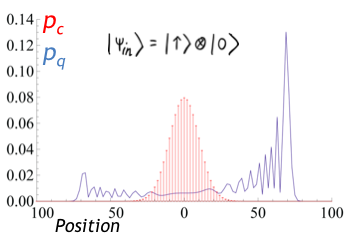
\includegraphics[width = 5cm]{pdf_zero_intial_state.png}
\end{figure}
\begin{figure}[ht]
    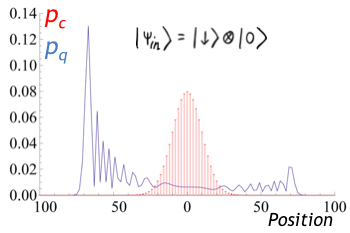
\includegraphics[width = 5cm]{pdf_zero_state1.png}
\end{figure}
\begin{figure}[b]
    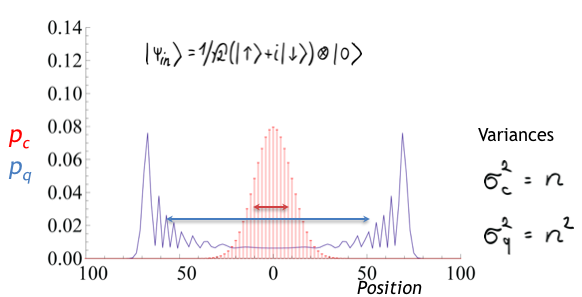
\includegraphics[width = 5cm]{pdf_symmetric.png}
\end{figure}
    
\end{frame}
\begin{frame}{Probability distribution}
\centering
\begin{figure}[htp]
    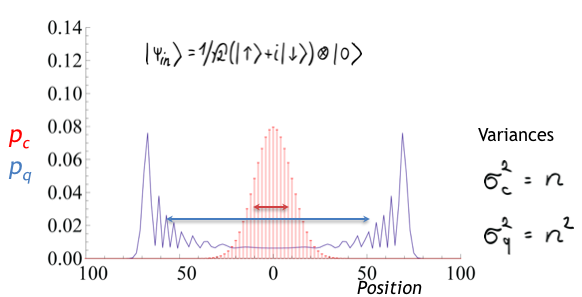
\includegraphics[width = 10cm]{pdf_symmetric.png}
\end{figure}
\end{frame}

\begin{frame}{Variance Compare }
\begin{figure}
    \centering
    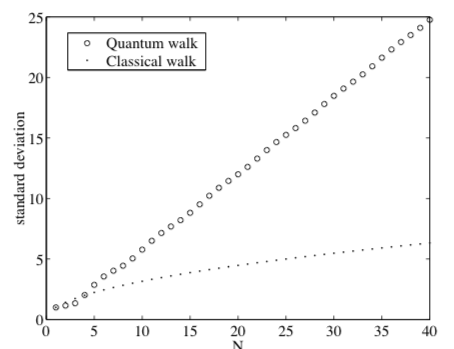
\includegraphics[width =6cm]{Variance_Comp.png}
    \caption{Standard deviation of quantum walk(circles) and classical random walk(dotes) against the number of steps}.
\end{figure}
\end{frame}

\begin{frame}{More on Quantum walk}
\textbf{Two state Case}
\begin{enumerate}
    \item Unitary matrix \begin{center}
     U = \begin{bmatrix}
                a & b\\
                c & d
         \end{bmatrix}
\end{center}
\item initial qubit states $$\Phi = \bigg\{\phi = \begin{bmatrix}
                    \alpha\\
                    \beta
                \end{bmatrix}
                \in \mathbb{C}^2 : \abs{\alpha}^2 + \abs{\beta}^2 =1\bigg\}
$$
\item we define two matrix P and Q :
$$P = \begin{bmatrix}
        a & b\\
        0 & 0
\end{bmatrix}, Q = \begin{bmatrix}
        0 & 0\\
        c & d
\end{bmatrix}$$
Remark that $$ U = P + Q$$.
\end{enumerate}
    
\end{frame}

\begin{frame}{Two state case}
\begin{enumerate}
    \item $$\phi_n(x) = \begin{bmatrix}
                \phi_{n}^L(x)\\
                \phi_{n}^R(x)
\end{bmatrix}   = \phi_{n}^L(x)\ket{L} + \phi_{n}^R(x)\ket{R} \in \mathbb{C}^2$$
and after N steps  $$ \phi_n = \begin{bmatrix}
        \phi_n(-N),\phi_n(-(N-1) \hdots \phi_n(N)
\end{bmatrix}$$
\item $$ \overline{U}_N = \begin{bmatrix}
                0 & P & 0 & \hdots & \hdots & 0 & Q\\
                Q & 0 & P & 0 & \hdots & \hdots & 0\\
                0 & Q & 0 & P & 0 & \hdots & 0\\
                \vdots & \vdots & \vdots & \vdots & \vdots & \hdots & \vdots\\
                0 & \hdots & 0 & Q & 0 & P & 0\\
                0 & \hdots & \hdots & 0 & Q & 0 & P\\
                P & 0 & \hdots & \hdots & 0 & Q & 0
\end{bmatrix}$$
\end{enumerate}
\end{frame}

\begin{frame}{Two state case}
$$  \phi_{n+1}(x) = (\overline{U}_N\phi_n)_x = P\phi_n(x+1) + Q\phi_n(x-1)$$
where $-N \leq x \leq N$ and $1 \leq n \leq N.$\\
\begin{enumerate}
    \item shift operator \begin{center}
    $S = \sum_{x \in \mathbb{Z}} \ket{x+1}\bra{x}$ and 
    $S^* = \sum_{x \in \mathbb{Z}} \ket{x-1}\bra{x}$
\end{center}
\item Unitary Operator $$  U = ( S \tens{} \Hat{Q} + S^* \tens{} \Hat{P})(I \tens{} H)$$
where $\Hat{P} = \ket{L}\bra{L}$ and $\Hat{Q}= \ket{R}\bra{R}$ are projection operator.
\item after n step the state is 
$$\phi_n = \overline{U}^n\phi_0$$
\end{enumerate}
\end{frame}

\begin{frame}{Possible Path Trajectory}
\begin{enumerate}
    \item fixed l and m with l+ m = n and -l + m = x
    $$ \Xi_n(l,m) = \sum_{l_j,m_j} P^{l_1}Q^{m_1} \hdots P^{l_n}Q^{m_n}  $$
satisfying $l_1 + l_2 + \hdots + l_n=l, m_1 + m_2+ \hdots +m_n = m$ and $l_j + m_j = 1$.\\
\textbf{Example}: for $P(X_4 =-2)$ the possible path is given by
$$  \Xi_n(3,1) = QP^3 + PQP^2 + P^2QP + P^3Q$$
\end{enumerate}
\end{frame}

\begin{frame}{Possible Path Trajectory}
We introduce two matrices R and S as
$$  R= \begin{bmatrix}
        c&d\\
        0&0
\end{bmatrix}, S=\begin{bmatrix}
    0&0\\
    a&b
\end{bmatrix}$$
we also note that
\begin{center}
\begin{tabular}{ c | c  c  c  c  }
   & P & Q & R & S\\
   \hline
  P & aP & bR & aR & bP\\
  Q & cS & dQ & cQ & dS\\
  R & cP & dR & cR & dP\\
  S & aS & bQ & aQ & bS
    \end{tabular}
\end{center}
this implies
$$\Xi_n(l,m) = p_n(l,m)P +q_n(l,m)Q +r_n(l,m)R + s_n(l,m)S $$
\end{frame}

\begin{frame}{Possible path Trajectory lemma}
\begin{figure}
    \centering
    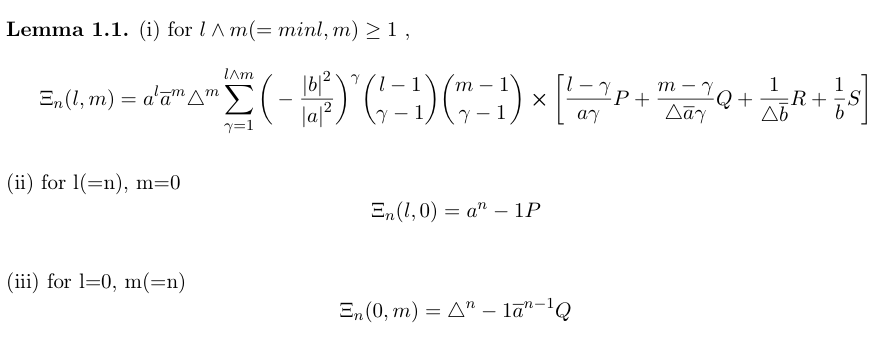
\includegraphics[width = 12cm]{Lemma1_1.png}
\end{figure}
\end{frame}

\begin{frame}{m-th order moment}
    \begin{figure}
    \centering
    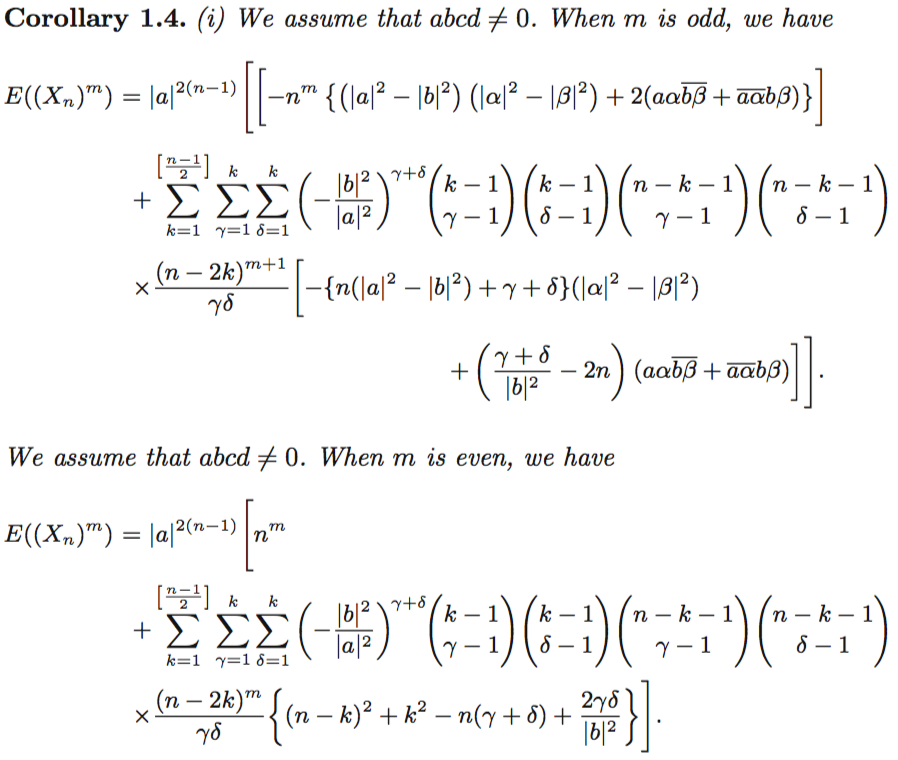
\includegraphics[width = 8cm]{Thm2.png}
\end{figure}
\end{frame}
\begin{frame}{m-th order moment}
    \begin{figure}
    \centering
    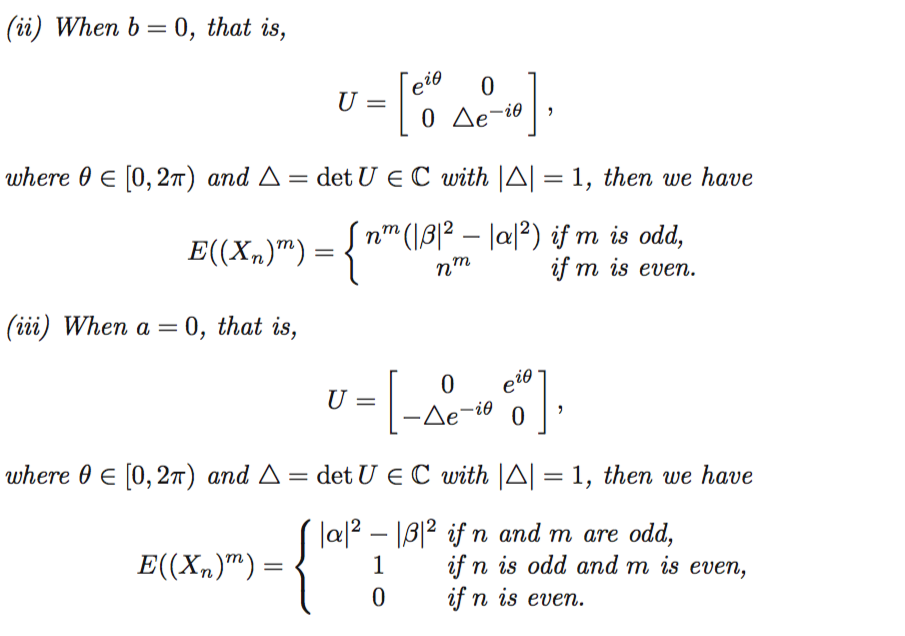
\includegraphics[width = 8cm]{Thm2_1.png}
\end{figure}
\end{frame}

\begin{frame}{Weak limit theorem}
\textbf{Theorem 1.5} If $n \rightarrow \infty$ , then 
                        $$ \frac{X_n}{n} \implies Z$$,
where Z has a density function\\

 $f(x) = f(x ; \phi = [\alpha, \beta]^T)
 = \dfrac{\sqrt{1-\abs{a}^2}}{\pi(1-x^2)\sqrt{\abs{a}^2 - x^2}}
 \bigg \{
 1-\bigg(\abs{\alpha}^2 -\abs{\beta}^2 +
 \dfrac{a\alpha\overline{b\beta} + \overline{a\alpha}b\beta}{\abs{a}^2}\bigg)x\bigg \}$, \\
 \\
 for $ x \in (-\abs{a},\abs{a}) and f(x) =  for \abs{x} \geq \abs{a}$ with\\
 $$E(Z) = -\bigg(\abs{\alpha}^2 -\abs{\beta}^2 + \dfrac{a\alpha\overline{b\beta} + \overline{a\alpha}b\beta}{\abs{a}^2}\bigg) \cross (1-\sqrt{1-\abs{a}^2})$$
 \hspace{3.25cm}$E(Z^2) = 1 - \sqrt{1-\abs{a}^2}$
    
\end{frame}

\begin{frame}{Plan of Actions}
\begin{enumerate}
    \item Multi-state case of Quantum walk
    \item Quantum analogue of Cellular Automata
    \item Quantum walk on cycles
    \item Absorbtion Problem
\end{enumerate}
    
\end{frame}

\begin{frame}{References}
\begin{enumerate}
 \item Norio Konno, Philiphe Biane, Quantum Potential Theory, Lecture Notes in Mathematics 2008
 \item J. Kempw. Quantum random walk:an introductory overview. Contemp. Phy. 2003
\item R. Portugal, Quantum walks and search algorithm Springer, 2013
\item A. Kitaev, A. Shen, and M. Vyalyi. Classical and Quantum Computation, volume 47 of Graduate Studies in Mathematics. American Mathematical Society, 2002.
\item Rieffel E.G. and Wolfgang H.P. quantum computing a gentle introduction.
\item M.A. Nielsen and I.L. Chuang Quantum computation and quantum information, Cambridge University Press, 2000.
\end{enumerate}
    
\end{frame}

\end{document}
